\chapter[Compositional exploration of fluid subspaces]{Compositional explorations of fluid subspaces}
\label{chap:chap6}

With our sonification system from Chapter \ref{chap:chap5} in hand, we now delve into its implications for composition. The process of musical composition, at its core, focuses on different
organizations of time. Commonly, we organize our thoughts and experiments on different timescales: the sound object level, which governs very short durations such as individual notes, the mesolevel, which is an intermediate scale which governs larger groups such as phrases or themes, and the macrolevel, which governs the overall form and structure of a piece of music. The idea of conceptualizing the
organization of music into three hierarchical time levels is especially emphasized in the works of Heinrich Schenker, whose theory of Schenkerian analysis works to unite the structure of musical pieces on the scales of 
foreground, middleground, and background \cite{cadwallader2007analysis}. Further subdivision of time scales have been noted by Curtis Roads, who articulates a total of nine time scales, ranging from the infinite down to the infinitesimal \cite{roads2004microsound}. While this more broad taxonomy is conceptually useful, in practice, composing a piece whose duration is only several minutes does not typically require working at time scales broader than our stated macro level. Additionally, unless the compositional process includes the use of ``microsound,'' or sounds that ``extend down to the threshold of auditory perception," we will also not need to work at time scales shorter than the sound object level. Hence, for our purposes, conceptualizing music in terms of three different time scales shall suffice.

\section{Mode Isolation}
The simplest compositional parameter of interest is the activation or deactivation of individual modes. While a physically accurate subspace re-simulation will, in general, at each time step, require a linear combination of each of the $r = 150$ modes, it is also possible to evolve the velocity fields over time according to algorithmic rules rather than physics-based rules. We imagine the $r$ modes as a sort of configuration space, so that the corresponding $r$ weights map to a particular spatial and aural phenomenon. As such, the most elementary experiment is the sequential activation of one mode at a time, creating a corresponding fluid shape of ``vibration'' which is mapped to its related ``frequency'' according to the system explained in Chapter 5. A low-\footnote{Low: \url{https://www.youtube.com/watch?v=CAoQLYr8doE}}  medium-\footnote{Medium: \url{https://www.youtube.com/watch?v=Vwpi6U7AD5A}} and high-frequency mode\footnote{High: \url{https://www.youtube.com/watch?v=o0UtONgtpFo}} are each shown isolated in the referenced videos. 

Because each mode in isolation can be regarded as a musical note, this strategy allows us to carry out musical composition on the note level, producing simple melodies. Without a principled way to choose a rhythm,
however, we are left only to general aesthetic considerations. An example of such a mode-based melody\footnote{Melody: \url{https://www.youtube.com/watch?v=N6fzJXbn2ts}} is demonstrated in the referenced video. (Figure \ref{fig:melody} shows a single 
frame from the video for reference.)

\section{Mode Superposition}
The next experiment to try is the superposition of modes, creating mixtures of the modal vibration shapes in the spatial domain and harmonies in the audio domain. Again, the physics-based time evolution governs a complex coupling of the modal weights that resists simple exploration, so we turn to simple algorithmic rules to better understand the system. We can see the result of mixing a low-, medium-, and high-frequency mode with equal proportions.

\begin{figure}[H]
	\centering
	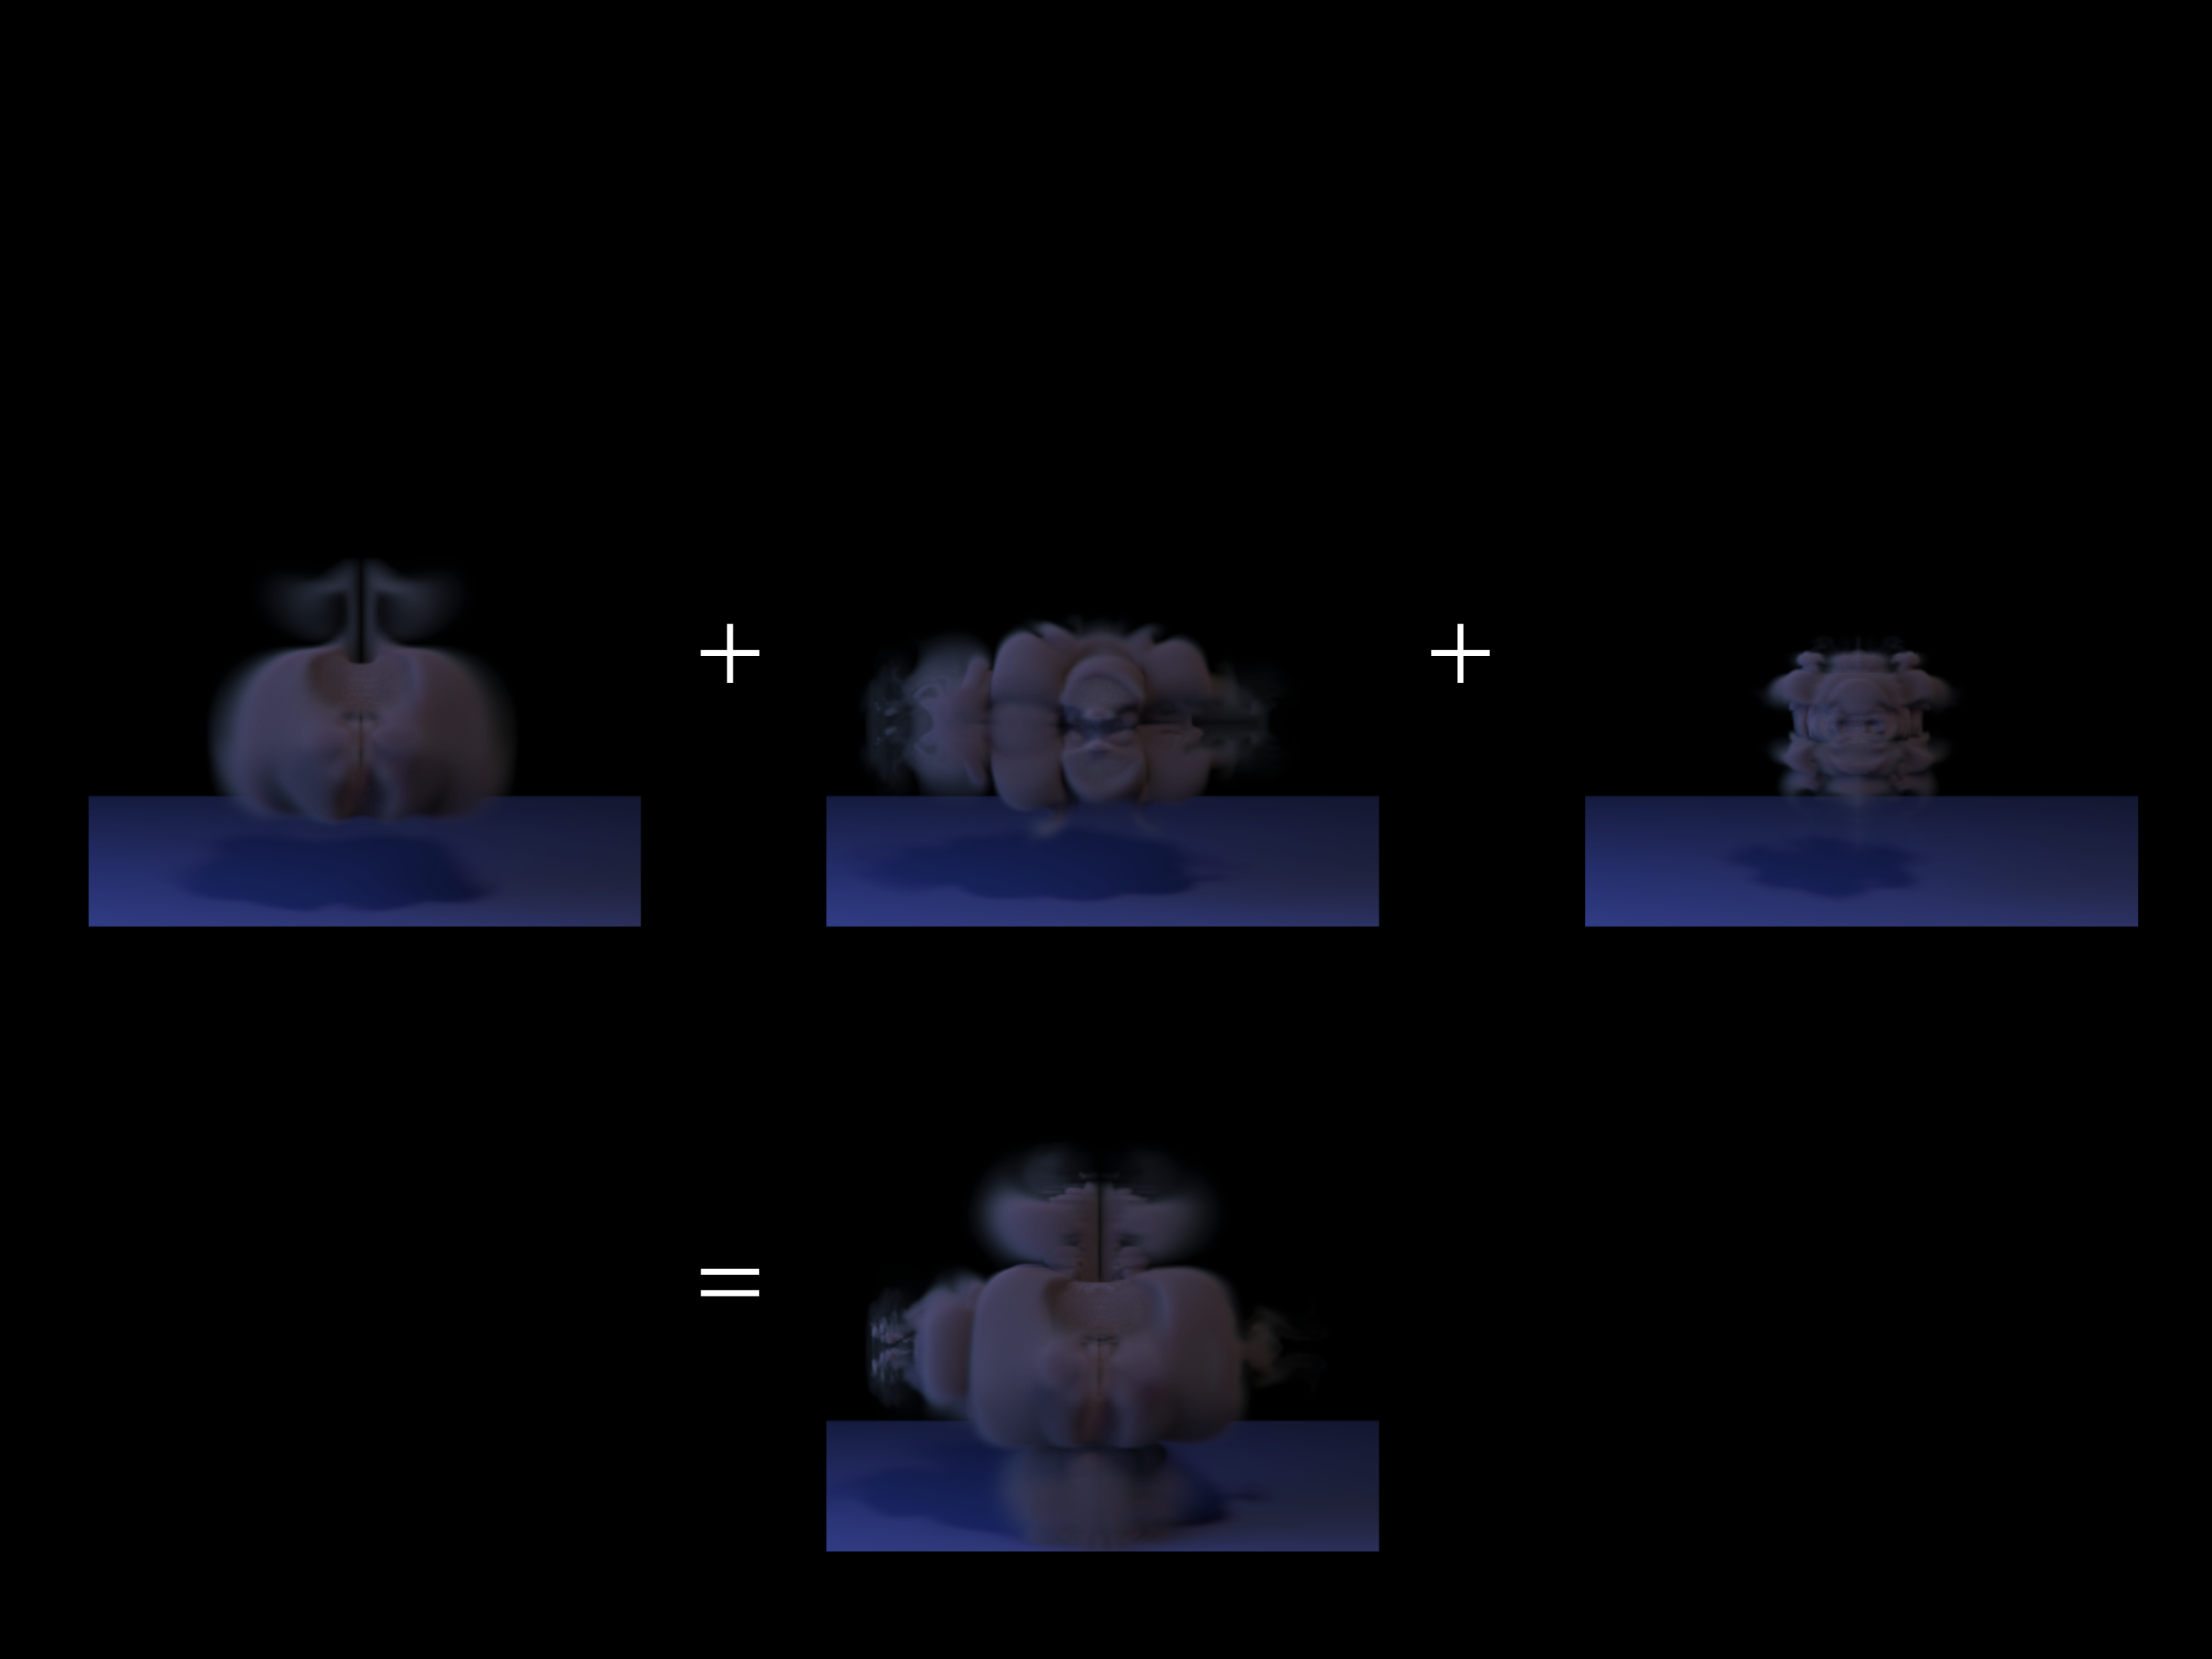
\includegraphics[width=\textwidth]{chap6/figures/superposition.png}
	\caption{\em Three individual modes in superposition produce a mixed modal shape.}
\label{fig:superposition}
\end{figure}

\section{Dynamic Control}
If we define the {\em energy} of a fluid snapshot in time as the $L_2$ norm of the vector of modal weights, then we see that as time unfolds, the energy waxes and wanes according to the strength
of the various modal weights. Accordingly, the sound increases or decreases in overall spectral density and loudness based on the same principle. However, by forgoing the physics-based time-evolution,
we can harness direct spectral control over the visuals and sound, producing simple and pleasing audiovisual gestures such as crescendo, diminuendi, and swells. An accent followed by diminuendo\footnote{Accent: \url{https://www.youtube.com/watch?v=0An95mF3Yk0}}, and a crescendo-diminuendo swell\footnote{Swell: \url{https://www.youtube.com/watch?v=zUkpNKpkwP4}} are each shown in the referenced videos, accompanied by still frames in Figures \ref{fig:dim} and \ref{fig:swell}, respectively.

\begin{figure}[H]
	\centering
	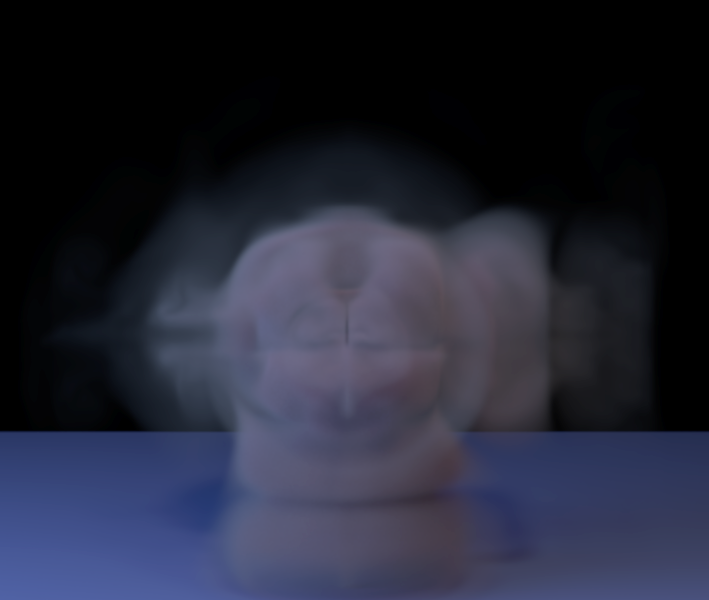
\includegraphics[width=\textwidth]{chap6/figures/dim.png}
	\caption{\em A still frame from the accent followed by diminuendo video.}
\label{fig:dim}
\end{figure}

\begin{figure}[H]
	\centering
	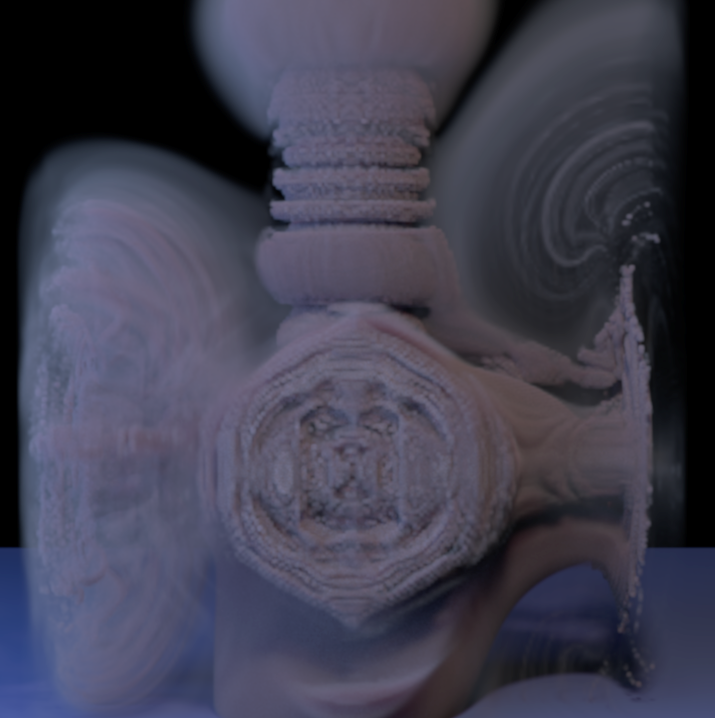
\includegraphics[width=\textwidth]{chap6/figures/swell.png}
	\caption{\em A still frame from the crescendo-diminuendo swell video.}
\label{fig:swell}
\end{figure}

\begin{figure}[H]
	\centering
	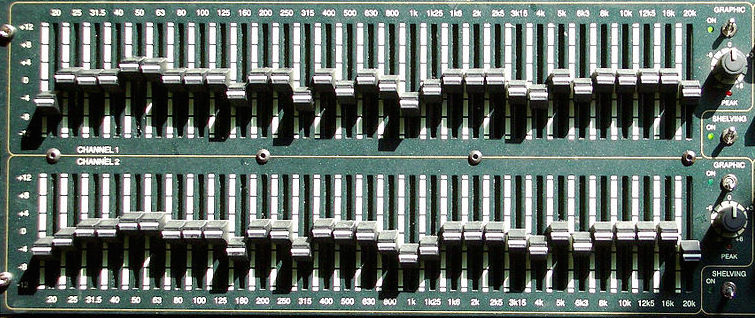
\includegraphics[width=\textwidth]{chap6/figures/faders.jpg}
	\caption{\em Each of the $r = 150$ modes can be controlled individually, analogous to a set of equalization faders. Source: Wikimedia Commons.}
\label{fig:faders}
\end{figure}

\section{Mode Coupling and Envelopes}
The simultaneous activation of all modes produces a spectrally rich sound quality, or timbre\footnote{According to ANSI 1960,
"Timbre is that attribute of auditory sensation in terms of which a listener can judge that two sounds similarly presented and having the same loudness and pitch are dissimilar. [. . .] Timbre depends primarily upon the spectrum of the stimulus."}, not dissimilar from noise. However, more refined filtering leads to a sparser spectrum, yielding a sound quality similar to musical chords. This filtering
can be achieved simply by activating only a small subset of the $r = 150$ modes at once, much as in the mode superposition study. However, such a chord is static over time, creating a dull musical effect for any prolonged 
duration. We can inject extra life into these chords by modulating their {\em envelopes}---i.e., creating time-varying amplitude envelopes around each mode. This strategy is akin to slowly adjusting the different fader knobs 
from high to low at different speeds. A simple mathematical collection of envelopes are sinusoids at different frequencies,\footnote{Oscillation: \url{https://www.youtube.com/watch?v=6nEVXFkWSZ4}} as the referenced video example illustrates. 
(Figure \ref{fig:osc} shows a single frame from this video for additional reference.) Visually, the shapes morph in and out of a slow cycle of superpositions, while the sound fades in and out of subtle frequencies of an overall chord.

\begin{figure}[H]
	\centering
	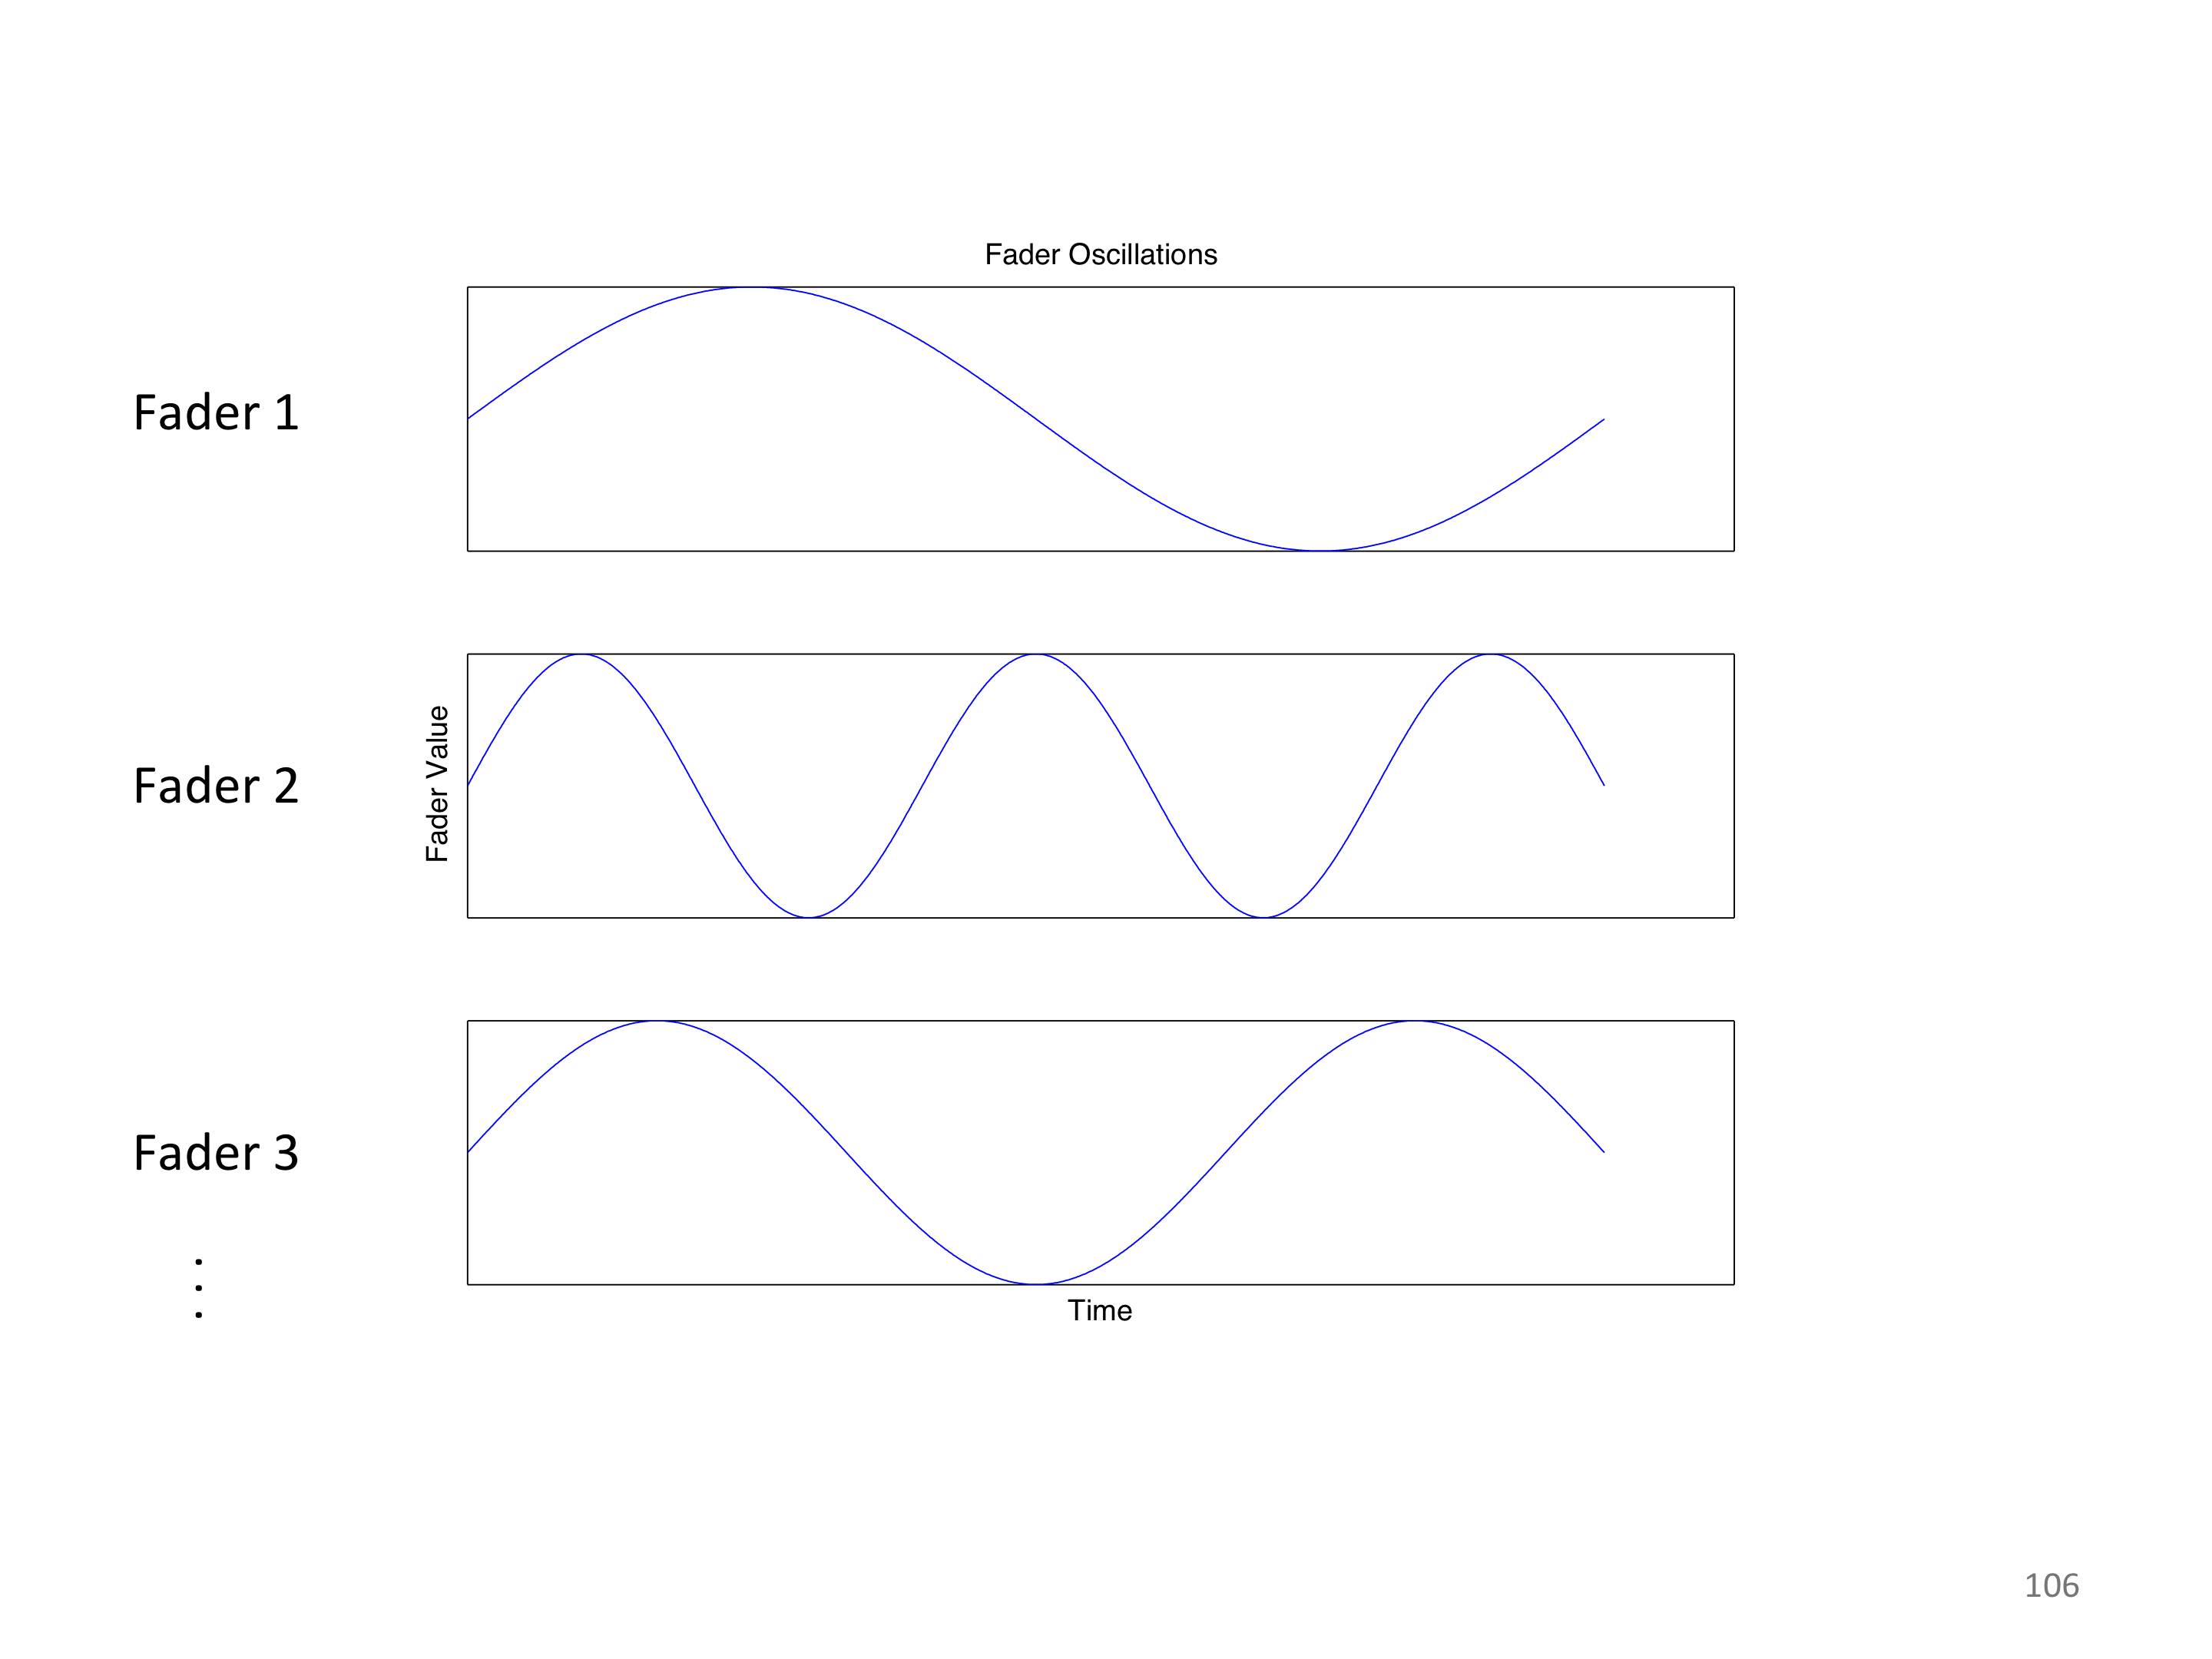
\includegraphics[width=\textwidth]{chap6/figures/fader_envelopes.png}
	\caption{\em Each modes's fader knob can be modulated smoothly over time, creating spectrally-varying envelopes.}
\label{fig:fader_envs}
\end{figure}

\begin{figure}[H]
	\centering
	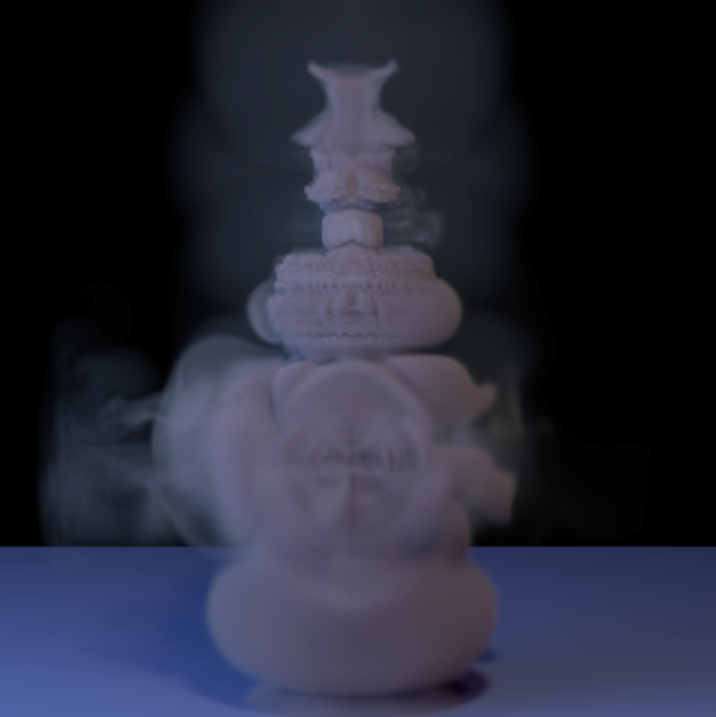
\includegraphics[width=\textwidth]{chap6/figures/osc.png}
	\caption{\em A single frame from the oscillation video generated by using time-varying sinusoidal envelopes of a chord.}
\label{fig:osc}	
\end{figure}

We can also {\em couple} different modes together, or transfer from one collection of modes smoothly into another, in analogy to a musical chord progression. (Coupling the modes is also inspired by the
complex nonlinear coupling induced by the real physical phenomenon of advection that we are simulating.) As time evolves, both the amplitude envelopes and the
spectral content itself shifts, producing a complex visual and audio effect\footnote{Crossfade: \url{https://www.youtube.com/watch?v=RCIuZaWqvds}} as seen in the referenced video example. (Figure \ref{fig:cross} shows 
a single frame from this video for additional reference.)

\begin{figure}[H]
	\centering
	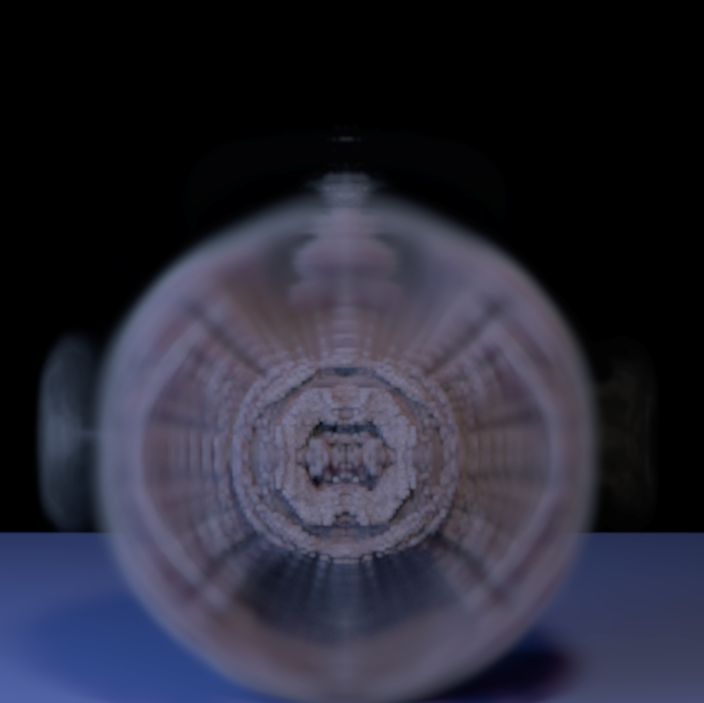
\includegraphics[width=\textwidth]{chap6/figures/cross.png}
	\caption{\em A single frame from the crossfade video generated by modulating both the amplitude envelopes and spectral content.}
\label{fig:cross}
\end{figure}

\section{Sonification Choices}
Now that we have seen the potential of our sonification system in action, we return to the justification of the many aesthetic choices made in designing it. We have an overwhelming freedom of choice here. In particular,  there is the choice of the physical training set, the choice of mapping between the dynamical system and the audio, and the choice of aesthetic stance. In the following sections, we will consider these issues in detail.

\subsection{Training Data}
Because our system relies on the empirical eigenvectors of a set of training data, the first choice we make in designing our system is the selection of the training data. An insufficiently rich training set will generate a series of results that are limited in dynamic variety due to the nature of the subspace algorithm. Early experiments in this direction were unsuccessful, as the collection of eigenvectors formed results that almost exactly mimicked the full-space simulation from which they were generated. Thus, the idea of using a sequence of full-space simulations was a natural attempt to mitigate this issue. However, since the eigenvectors are agnostic to time, it is useful to construct a sequence of simulations that are very distinct from one another. Hence, our strategy of modifying the direction of buoyancy was appealing. This technique results in six different outward-facing plumes, each of which having its own unique dynamics. The inherent symmetry to this strategy is also appealing from an aesthetic standpoint, as by privileging no one direction over another, the eigenvectors acquire a more abstract quality, detaching them from the more scientifically-grounded full-space simulation. As a result, the empirical eigenvectors take on a series of aesthetically pleasing turbulent forms, ideally suited for generating novel audiovisual compositions.

\subsection{Sound Synthesis}
As discussed in Chapter \ref{chap:chap2}, the details in implementing a system of sonification allow for a wide freedom of choice. Hence, it is important to justify our choices by perceptual or aesthetic concerns. We identify and discuss several of our choices in this section.

Perhaps the choice that influences most the character of our auditory results is our choice for sound synthesis. No matter what mapping we choose from physics to sound, the engine which produces actual audible sound influences the output tremendously. Thus, our choice of using subtractive synthesis of spectrally rich noise deserves further investigation. Indeed, our initial concept utilized a simpler system of additive synthesis. However, we found the subtractive synthesis more suitable to our aesthetic needs for several reasons.

Firstly, our system produces not just sound, but sound and visuals. Aesthetically speaking, we desired a reasonable congruence between the character of both the audio and the visual domain. In particular, although the dynamics of the visuals varied substantially, the overall look and feel did not---the simulations were all fluid dynamics of smoke billowing about smoothly. Thus, we immediately discarded many audio results that were choppy and robotic, as the resulting incongruence was displeasing aesthetically. We also discarded a quantized scale such as 12-tone equal temperament, feeling that its rigidity would belie the abstract amorphous quality of our visuals. Therefore, what remained to explore were ambient, textural sounds. Both additive and subtractive synthesis seemed promising, as we had in hand a collection of frequencies from our mapping scheme. While additive synthesis is simple and effective, its results tend to be too sterile for our taste. The individual sinusoids are too digitally clean, and their superpositions result in a computer-like purity that also belies the messy, turbulent swirls of our visuals. Hence, we turned our attention to subtractive synthesis. As discussed in Chapter \ref{chap:chap2}, in some sense, subtractive synthesis is a logical choice, as the entire concept of modes of vibration that our sonification system depends on is built on the foundation of subtractive synthesis. Moreover, by varying the input signal to the filter, a variety of different timbres can be generated. In contrast, additive synthesis produces one single result, which must then be additionally filtered and adjusted to produce pleasing outputs. We settled on using gray noise, which emphasizes the lower frequencies in its spectral output, to bring out the principal singular values more prominently \cite{wilson2011supercollider}. It must be mentioned that the choice itself to map the principal singular values to lower frequencies---that is, a choice of polarization, as discussed in Chapter \ref{chap:chap2}, is itself somewhat arbitrary. However, this choice rests on perceptual considerations, not aesthetic ones. The prominent sonic tones in any timbre are the fundamental frequencies, which are the lowest frequencies; hence, inverting the singular values to match this prominence is a natural and justifiable step to take.

\subsection{Real-Time and Non-Real-Time Strategies}
One of the potential drawbacks of our audiovisual system is its heavy computation cost. As a result, the capacity for real-time interaction is infeasible as of time of writing in 2017. However, the dynamics of non-real-time composition allow for a different 
type of compositional process than a real-time system would afford. In this section, we discuss a few pros and cons of each of these types of systems, illustrating our non-real-time approach while suggesting a roadmap to eventual real-time strategies.

By its nature, a non-real time system lends itself better toward careful structural planning. Pieces must be planned and executed ahead of time rather than as a flash of inspiration. Hence, formal structures flourish, and strategies for unifying a
piece on different time scales become very attractive. The possibility of unifying the material of a piece in the micro-, meso-, and macro-time scales is aesthetically powerful, and only possible through non-real-time composition. As a result, pieces that
are designed with a non-real-time process tend to be structurally sound and aesthetically coherent.

However, the high degree of structure of non-real-time strategies can also be a weakness. The capacity for free improvisation and interaction through real-time often produces unexpected and daring results. Feedback through interaction with the system and having the system ``interact back'' can be extremely rewarding, leading to new insights and promising directions that would otherwise be impossible to discover. Additionally, the ability of the audience to participate in a piece through interaction changes the very nature of the piece. A viewer/listener no longer must let the experience wash over them; instead, they participate actively in the creation of the piece themselves, defining their own new experience which is distinct from all other viewers' experiences.

Ultimately, the non-real-time strategies employed in this dissertation proved effective, as the audiovisual studies were only possible from designing a careful strategy of moving through the subspace according to either mathematical or physical rules. However, the capacity for a real-time interaction to generate unexpected new insights and results from this system remains to be seen, and is a promising direction for future work. Interaction could happen on many levels. For example, the interaction could adjust physical parameters, by introducing new obstacles to the simulation or adjusting the buoyancy or vorticity of the flow. Alternatively, the interaction could be more gestural, allowing the user to control the energy of the system, creating dynamical swells and frequency sweeps as demonstrated by the earlier studies in this section. 

\subsection{Aesthetics}
In our creation of these studies, we imposed our own aesthetic values to some degree on the sonification system to produce musical results. While some sonifications remain purely scientific, created only for the purpose of identifying patterns in data, our own system was always born out of a desire to create musical outputs. The tension between adhering to fixed scientific principles and generating aesthetically interesting musical output is  a constant challenge in composing generative music of this kind. Our aesthetic take, as discussed in Chapter \ref{chap:chap2}, is a middleground between these two extremes. While a system itself can be aesthetically pleasing in the mathematical sense, this is no guarantee of the quality of its musical output. Conversely, a total abandonment of the systematic approach simply for the reasons of adjusting the musical output largely negates the point of composing using such a system in the first place. To that end, our musical adjustments remained of a minor quality, not abandoning the logic of the system, but merely adjusting it in certain cases to compensate for the quality of the musical output. For example, when we take our amplitude mapping from the numerical data of the simulation, all sign information is neglected, as a positive and negative amplitude in sound merely represents an unpleasant phase distortion. While this approach arguably throws away a dimension of the physical data, it does not fundamentally detach the result from the system, and is thus considered acceptable from our aesthetic point of view.

One of our principal aesthetic goals toward future work is the idea of simulating smoke under more fanciful systems of time-evolution than standard physics. Hence, many of our examples play with the idea of controlling the time evolution in different mathematical procedures rather than sticking with the correct physics. While this again is pushing the boundaries of our original system, we nonetheless retain the same link between the visual and audio results. Thus, we view this form of modulation as
a robust way to explore new compositional forms. Changing the underlying rules which govern the time-to-time behavior of the audiovisual system is not the same as abandoning the system; in fact, it has proved fruitful in generating novel results. These strategies move us more in the direction of simulating fluids ``as they might be'' vs. fluids ``as they actually are.''